% !TeX spellcheck = de_DE
\documentclass[10pt, a4paper]{amsart}
\usepackage[utf8x]{inputenc}
\usepackage{polyglossia}
\setdefaultlanguage{ngerman}
\usepackage{enumitem}

\usepackage{xcolor}

\usepackage{caption}
\captionsetup[figure]{name=Abbildung}
\usepackage{tikz, tkz-euclide}
\usetikzlibrary{calc}

\usepackage{amsmath, amsfonts, amssymb}
\usepackage{amsthm, thmtools}
\declaretheorem[name=Aufgabe, thmbox = L]{aufgabe}
\declaretheorem[name=Lemma]{lemma}
\counterwithin*{lemma}{aufgabe}
\counterwithin*{equation}{aufgabe}
\newcommand{\aufgabelabelname}{\theaufgabe . Aufgabe}
\renewcommand\qedsymbol{$\blacksquare$}
\renewcommand\proofname{Beweis}

\usepackage{physics}
\usepackage{fancyhdr}
\pagestyle{fancy}
\fancyheadoffset{0cm} 
\usepackage[
  a4paper,
  right=6cm,
  footskip=3em,
  twoside=false,
  lmargin=1.4cm,
  xetex,
]{geometry}
\usepackage{unicode-math}
\listfiles
\makeatletter
\renewenvironment{proof}[1][\proofname]{\par
\pushQED{\qed}%
\normalfont \topsep6\p@\@plus6\p@\relax
\trivlist
\item\relax
{\bfseries#1}\hspace\labelsep\ignorespaces
}{%
\popQED\endtrivlist\@endpefalse
}
\newenvironment{proof_thm}[1]{
\begin{proof}[\proofname~(#1)]}{\end{proof}}
\makeatother

\chead{
	\fontsize{9}{7}\large\aufgabelabelname
}
\rhead{
	\fontsize{9}{7}Valentin Herrmann}

%  \begin{tikzpicture}
%      \def\range{41}%
%      \def\radius{0.6cm}%
%      \def\a{\fpeval{360/\range}}%
%      \foreach \i in {0,1,...,\range}{%
%        \definecolor{colora}{hsb}{\fpeval{\i/\range},1,0.7}%
%        \draw[colora, very thin] (\i*\a-90:\radius) -- (2*\i*\a-90:\radius);%
%      }%
%      \draw[very thin] (0,0) circle[radius=\radius];%
%    \end{tikzpicture}

%hyperref must be the last package in the preamble
\usepackage{hyperref}
\hypersetup{
	bookmarks=true,
	unicode=true,
	pdfborder={0 0 0},
	pdfstartview={FitH},
	pagebackref=true,
	colorlinks=true,
	urlcolor=blue,
	linkcolor=black,
	linktoc=all
}
\renewcommand{\figureautorefname}{Abbildung}

\begin{document}
\thispagestyle{fancy}
\begin{aufgabe}
  Leo und Smilla finden 2020 Goldnuggets mit den Massen 1, 2, ..., 2020 Gramm,
  die sie nach folgender Regel auf eine rote und eine blaue Schatztruhe
  verteilen:
  
  Zuerst wählt Leo eine der Schatztruhen und nennt Smilla die Farbe der Truhe.
  Anschließend wählt Smilla eines der noch nicht verteilten Nuggets und legt es
  in diese Truhe. Dies wiederholen sie, bis alle Nuggets verteilt sind. Danach
  wählt Smilla eine der beiden Schatztruhen und bekommt alle Nuggets in dieser
  Truhe.

  Wie viel Gramm Gold kann Smilla auf diese Weise mindestens für sich
  garantieren?
\end{aufgabe}
\begin{lemma}\label{sec1:Zahlensumme}
  Es gilt für alle $n∈ℕ^*$:
  \[ \sum^{n}_{k=1}k=\dfrac{n(n+1)}{2}\]
\end{lemma}
\begin{lemma}
  \label{sec1:zahlengruppen}
  Jeder Abschnitt der natürlichen Zahlen, welcher mit 1 beginnt und mit einer
  Zahl $n=4k+3$, $k∈ℕ_0$ aufhört, kann in zwei gleich große Gruppen geteilt
  werden.
\end{lemma}
\begin{proof}
  Für einen einfacher lesbaren Beweis werden die Nuggets jeweils nach ihrer
  Masse benannt. Nugget $1234$ steht also für das Nugget mit der Masse $1234$g.
  Zusätzlich werden einige Variablen nach dem entsprechenden Zeitpunkt bennant.
  Zum Beispiel steht $r_{2019}$ für das Gewicht der roten Truhe nach der Vergabe
  des 2019ten Nuggets mit einem Gewicht von $n_{2019}$.
  
  Zuerst wird die Obergrenze für Smillas maximalen Schatz bestimmt. Vor der
  Vergabe des letzten Nuggets entspricht die Summe des Gewichts beider Truhen
  der Summe aller Nuggets bis auf Nugget $n_{2020}$. Als Gleichung geschrieben
  unter Anwendung von ~\autoref{sec1:Zahlensumme}:
  \begin{equation}\label{sec1:equation1}
    r_{2019}+b_{2019}=\sum_{k=1}^{2020}\left(k\right)-n_{2020}=\dfrac{2020\cdot2021}{2}-n_{2020}
  \end{equation}
  Da Smilla sich nach der Aufteilung ihre Truhe aussuchen darf wird Leo die
  leichtere Truhe bekommen. Daher wird Leo versuchen die Truhen
  so gleichmäßig wie möglich zu füllen. Daher wird Leo logischerweise die
  leichtere Truhe für das letzte Nugget wählen.

  Angenommen es gilt $r_{2019}\leq b_{2019}$ vor der Vergabe des letzten Nuggets (Die Truhen sind
  austauschbar), dann wird Leo die rote, leichtere Truhe wählen und Smilla wird das letzte
  Nugget $n_{2020}$ in diese Truhe legen. Daraus folgt mit~\eqref{sec1:equation1}:
  \begin{equation}\label{sec1:equation2}
    r_{2020}=r_{2019}+n_{2020}=(1010\cdot2021-b_{2019}-n_{2020})+n_{2020}=1010\cdot2021-b_{2019}
  \end{equation}
  Also hat $r_{2020}$ den maximalen Wert, wenn $b_{2019}$ minimal ist. Da
  $b_{2019}$ größer gleich $r_{2019}$ sein muss, ist der minimale Wert von
  $b_{2019}$ gleich $r_{2019}$. Für den Idealfall $r_{2019}=b_{2019}$ folgt daher
  mit~\eqref{sec1:equation1}:
  \begin{equation}\label{sec1:equation3}
    \begin{split}
      b_{2019} + r_{2019}= 2b_{2019} &=1010\cdot2021-n_{2020}\\
      \Rightarrow b_{2019} &=505\cdot2021-\dfrac{n_{2020}}{2}
    \end{split}
  \end{equation}
  Wird~\eqref{sec1:equation3} in \eqref{sec1:equation2} eingesetzt:
  \begin{equation*}
    r_{2020}=505\cdot2021+\dfrac{n_{2020}}{2}
  \end{equation*}
  Im Idealfall für Smilla ist $n_{2020}$ maximal groß und hat daher den Wert
  2020. Damit gilt für die Obergrenze $r_{2020}$:
  \begin{equation*}
    r_{2020}=505\cdot2021+1010 = 505\cdot2023 = 1021615
  \end{equation*}
  Nun stellt sich die Frage, ob Smilla diese Obergrenze überhaupt erreichen
  kann. Eine Strategie für Smilla um mindestens die Obergrenze von $1021615$ zu erreichen ist Folgende:

  Smilla trennt alle Nuggets bis auf $2020$ in zwei gleich schwere Gruppen.
  Das ist möglich, da dar größte Nugget $2019$ gleich $4\cdot504 + 3$ ist,
  weshalb~\autoref{sec1:zahlengruppen} anwendbar ist. Jede Gruppe entspricht
  dabei einer Truhe. Wählt nun Leo eine Truhe aus, so legt Smilla ein Nugget aus
  der entsprechenden Gruppe hinein. Wählt Leo irgendwann eine Truhe aus, in
  welcher schon alle Nuggets der entsprechenden Gruppe sind, so legt Smilla das
  Nugget 2020 in diese Truhe, womit die Obergrenze erreicht ist:
  \begin{equation*}
    \frac{\sum_{k=1}^{2019}}{2}
    + 2020 = \frac{\frac{2019\cdot2020}{2}}{2} + 2020 = 2019\cdot505 + 4\cdot505 =
    2023\cdot505 = 1021615
  \end{equation*}
\end{proof}
\begin{proof_thm}{\autoref{sec1:Zahlensumme}}
  \begin{align*}
    \sum^{n}_{k=1}k&=\dfrac{1}{2}\cdot\left( \sum^{n}_{k=1}k +
                     \sum^{n}_{k=1}(n+1-k)\right) = \dfrac{1}{2}\cdot\sum^{n}_{k=1}(k+(n+1-k))\\
                   &=\dfrac{1}{2}\cdot\sum^{n}_{k=1}(n+1) = \dfrac{n(n+1)}{2}
  \end{align*}
\end{proof_thm}
\begin{proof_thm}{\autoref{sec1:zahlengruppen}}
  Die Zahlenreihe wird um Null erweitert, sodass die Reihe aus insgesamt
  $n+1=4(k+1)$ Zahlen besteht. Nun wird die Zahlenfolge in der Mitte „gefaltet“.
  Die kleinste Zahl wird mit der Größten gepaart, die zweit Kleinste mit der
  zweit Größten, etc. So enstehen $\frac{4(k+1)}{2}=2(k+1)$ Paare, jeweils mit
  einer Summe von $(j)+(n-j) = n$ mit $j∈ℕ_0$ und $0\leq j \leq n$. Da die Paare
  alle gleich groß sind und es eine gerade Anzahl von ihnen gibt, können sie in
  zwei gleich große Gruppen mit gleich vielen Paaren unterteilt werden. Dabei
  kann nun die Null wieder entfernt werden, schließlich verändert sie die Summen
  ihrer Gruppen nicht.
\end{proof_thm}

\newpage
\begin{aufgabe}
  Beweise: Es gibt keine rationalen Zahlen $x$, $y$, $z$ mit $x + y + z = 0$ und
  $x + y + z = 100$.
\end{aufgabe}
\begin{lemma}\label{sec2:rational1}
  Jeder Quotient $\frac{a}{b}$ zweier rationaler Zahlen $a,b∈ℚ\backslash\{0\}$
  ist rational definiert.
\end{lemma}
\begin{lemma}\label{sec2:rational2}
  Jedes Produkt $ a\cdot b $ einer rationalen Zahl $a$ ungleich Null und einer
  irrationalen Zahl $b$ ist irrational definiert.
\end{lemma}
\begin{proof}
  Angenommen es könne rationale Zahlen $x$, $y$, $z$ mit $x + y + z = 0$ und
  $x + y + z = 100$ geben.
  
  Zuerst wird $x+y+z = 0 \Rightarrow z = -(x+y)$ in $x^2+y^2+z^2 = 100$
  eingesetzt. Also gilt:
  \begin{equation}
    \label{eq:1}
    \begin{split}
      x^2+y^2+(-(x+y))^2 = x^2+y^2+(x^2+2xy+y^2) &= 100\\
      \Rightarrow x^2+xy+y^2&=50
    \end{split}
  \end{equation}
  Hieraus folgt direkt, dass $x$ und $y$ nicht gleich Null sein können. Wären sie
  beide Null, so gilt $0^2+0\cdot0+0^2=0=50$, was nicht gelten kann. Ist nur eine der Variablen
  Null so gilt: $0^2+0\cdot a+a^2=a^2=50\Rightarrow a = \pm5\sqrt{2}$. $a$ ist
  dabei ein Platzhalter für $x$ oder $y$. Da $\sqrt{2}$ irrational ist, ist
  nach~\autoref{sec2:rational1} auch dieser Fall nicht möglich, sonst wäre $a$
  schließlich irrational.

  Durch Teilen von~\eqref{eq:1} durch $x^2$ entsteht
  $(\frac{y}{x})^2+\frac{y}{x}+1=\frac{50}{x^2}$. Das Teilen durch $x^2$ ist
  erlaubt, da $x$ nicht Null sein kann.
  
  Aus~\autoref{sec2:rational2} folgt, dass $\frac{y}{x}$ als eine gekürzte
  rationale Zahl $\frac{m_q}{n_q}$ mit $m_q,n_q\in\mathbb{Z}\backslash\{0\}$,
  beschreibbar sein muss. Auch $x$ muss
  als rationale Zahl $\dfrac{m_x}{n_x}$, mit
  $m_x,n_q\in\mathbb{Z}\backslash\{0\}$ beschreibbar sein.
  Also kann die Gleichung umgeschrieben werden:
  \begin{equation}
    \label{eq:2}
    \begin{split}
      \left(\dfrac{m_q}{n_q}\right)^2+\dfrac{m_q}{n_q}+1&=\dfrac{50}{\left(\frac{m_x}{n_x}\right)^2}=\dfrac{2\cdot 5^2n_x^2}{m_x^2}\\
      \Rightarrow \dfrac{m_q^2+m_q\cdot n_q +
        n_q^2}{2}&=\dfrac{5^2n_x^2n_q^2}{m_x^2}=\left( \dfrac{5n_xn_q}{m_q}
      \right)^2
    \end{split}
  \end{equation}
  Da die rechte Seite von~\eqref{eq:2} das Quadrat einer rationalen Zahl ist,
  gilt dies auch für $\frac{m_q^2+m_q\cdot n_q + n_q^2}{2}$. Da Qudrate von
  rationalen Zahlen bei allen ihren Primfaktoren gerade Exponenten haben, muss
  gleiches für die linke Seite, insbesondere für den Primfaktor $2$ gelten. Doch
  solange der Zähler der linken Seite nicht durch zwei teilbar ist, hat 2 bei
  ihr einen ungeraden Exponent von $-1$. Daher wird zwischen drei Fällen unterschieden:
  \begin{itemize}[itemsep=2ex]
  \item Sind $m_q$ und $n_q$ beide ungerade:
    \[m_q^2+m_qn_q+n_q^2\equiv1^2+1\cdot1+1^2\equiv1\pmod{2}\] In
    diesem Fall ist der Zähler ungerade, weshalb die
    linke Seite kein Qudrat einer rationalen Zahl sein kann. Es gibt einen
    Widerspruch.
  \item Ist $m_q$ gerade und $n_q$ ungerade:
    \[m_q^2+m_qn_q+n_q^2\equiv0^2+0\cdot1+1^2\equiv1\pmod{2}\] Auch hier ist
    wird der Zähler ungerade, womit gleiches wie im vorherigen Fall gilt.
  \item Da der Zähler symmetrisch in Rücksicht auf $m_q$ und $n_q$ ist, gilt
    wenn $m_q$ ungerade und $n_q$ gerade ist, gleiches wie im vorherigen
    Fall.
  \item Es können nicht beide Variablen gerade sein, da sie nach der Definition teilerfremd sein müssen.
  \end{itemize}
  Also kann die linke Seite der Gleichung kein Quadrat einer rationalen Zahl
  sein. Es entsteht ein Widerspruch. Also kann $\frac{y}{x}$ keine rationale Zahl sein, wenn $x$ eine rationale
  Zahl ist. Doch gleichzeitig folgt aus~\autoref{sec2:rational1}, dass
  $\frac{y}{x}$ eine rationale Zahl sein muss, wenn $x$ und $y$ rational sind.
  Daher können $x$ und $y$ nicht beide rational sein.
\end{proof}
\begin{proof_thm}{\autoref{sec2:rational1}}
  Wird $a$ durch $\frac{m_a}{n_a}$ und $b$ durch $\frac{m_b}{n_b}$ beschrieben,
  wobei $m_a,n_a,m_b,n_b∈ℕ^*$ gilt, so kann der Quotient $\frac{a}{b}$ als
  $\frac{\frac{m_a}{n_a}}{\frac{m_b}{n_b}}=\frac{m_a\cdot n_b}{m_b\cdot n_a}$
  geschrieben werden. Da $m_a\cdot n_b$ und $m_b\cdot n_a$ ganze Zahlen ungleich
  Null sind, muss der Quotient rational sein.
\end{proof_thm}
\begin{proof_thm}{\autoref{sec2:rational2}}
  Beweis durch Widerspruch: Angenommen das Produkt $c$ ist eine rationale Zahl:
  \begin{equation*}
    ab=c \Rightarrow b =\frac{c}{a}
  \end{equation*}
  Die rechte Seite muss nach~\autoref{sec2:rational1} rational sein, also darf
  $b$ nicht irrational sein.
\end{proof_thm}

\newpage
\begin{aufgabe}
  Zwei Geraden $m$ und $n$ schneiden sich in genau einem Punkt $P$. Ein Punkt
  $M$ bewegt sich auf m mit konstanter Geschwindigkeit, ein weiterer Punkt $N$
  bewegt sich auf $n$ mit derselben Geschwindigkeit; dabei passieren sie beide
  den Punkt $P$, aber nicht gleichzeitig.
 
  Beweise: Es gibt einen festen, von $P$ verschiedenen Punkt $Q$ so, dass die
  Punkte
  $P$, $Q$, $M$ und $N$ zu jedem Zeitpunkt auf einem gemeinsamen Kreis liegen.\\
\end{aufgabe}
\begin{lemma}\label{sec3:lemma1}
  Für jeden festen Punkt $P$ und $Q$ existiert ein Gerade $g$, sodass
  der Mittelpunkt von jedem Kreis, welcher durch beide Punkte führt, auf der
  Geraden liegt.
\end{lemma}
\begin{lemma}\label{sec3:lemma3}
  Für jeden Punkt $P$ und jede Gerade $g$ existiert ein Punkt $Q$, sodass jeder
  Kreis, dessen Mittelpunkt auf der Geraden liegt und auf welchem $P$ liegt,
  auch durch $Q$ führt
\end{lemma}
\begin{lemma}\label{sec3:lemma2}
  Sind in einem Dreieck zwei Höhen gleich, so muss das Dreieck gleichschenklig
  sein. Dabei sind die Seiten auf welchen die Höhen stehen die Schenkel des
  gleichschenkligen Dreiecks.
\end{lemma}
\begin{proof}
  Nur exakt dann wenn alle $U$ auf der gleichen Geraden
  liegen, existiert nach~\autoref{sec3:lemma1} ein weiterer Punkt außer $P$,
  welcher für alle verschiedenen $U$ auf dem Kreis liegt.

  Um das zu beweisen wird nun das lose $U_t$ mit einem festen $U_0$ verglichen. Der
  Umkreismittelpunkt eines Dreiecks kann als Schnittpunkt der
  Mittelsenkrechten der Dreiecksseiten konstruiert werden. Zwei Mittelsenkrechten reichen
  dabei aus:
  
  \begin{figure}[h]
    \centering
    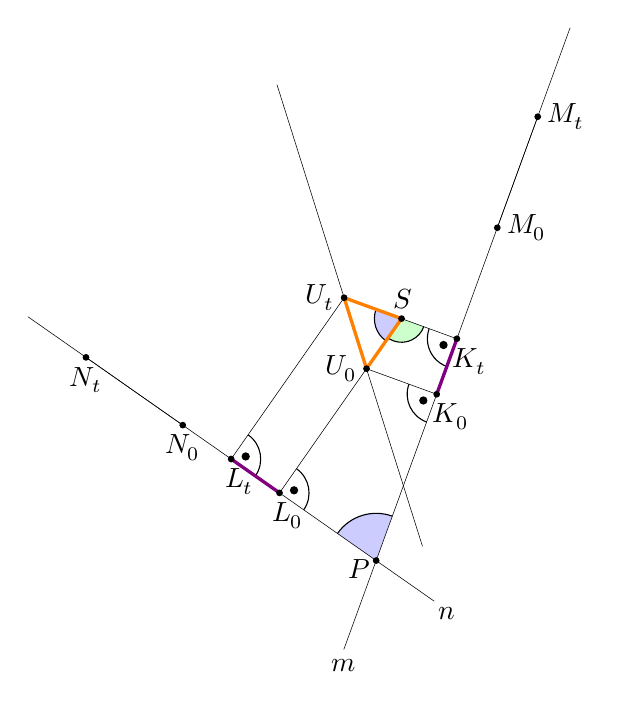
\begin{tikzpicture}[rotate=70,scale=1.5]
      % \tkzSetUpLine[add=.5 and .5]%
      \tkzSetUpPoint[fill=black]%
    
      \def\vara{75} \def\varx{1}%
    
      \tkzDefPoint(0,0){P} \tkzDefPoint(0:4){M_t} \tkzDefPoint(\vara:3){N_t}%
      \tkzDefShiftPoint[M_t](0:-\varx){M_0}%
      \tkzDefShiftPoint[N_t](\vara:-\varx){N_0}%

      \foreach \i in {0, t} { \foreach \kl/\mn in {K/M, L/N} {%
          \tkzDefLine[mediator](P,\mn_\i) \tkzGetPoints{\kl_\i_1}{\kl_\i_2}%
          \tkzInterLL(\kl_\i_1,\kl_\i_2)(P,\mn_\i) \tkzGetPoint{\kl_\i} }%
        \tkzInterLL(K_\i_1,K_\i_2)(L_\i_1,L_\i_2) \tkzGetPoint{U_\i} }%

      \tkzInterLL(L_0_1,L_0_2)(K_t_1,K_t_2) \tkzGetPoint{S}%
      % \tkzInterLL(K_0_1,K_0_2)(L_t_1,L_t_2) \tkzGetPoint{R}%

      \tkzFillAngles[fill=blue!20,size=0.4](M_t,P,N_t)%
      \tkzFillAngles[fill=green!20,size=0.2](U_0,S,K_t)%
      \tkzFillAngles[fill=blue!20,size=0.23](U_t,S,U_0)%
      
      \tkzMarkAngle[size=0.4](M_t,P,N_t)%
      \tkzMarkAngle[size=0.2](U_0,S,K_t)%
      \tkzMarkAngle[size=0.23](U_t,S,U_0)%
      \tkzMarkRightAngles[german](P,L_t,U_t P,L_0,U_0 U_t,K_t,P U_0,K_0,P)%

      % \tkzDefLine[parallel=through L_t](L_0,S) \tkzGetPoint{L_t'}%
      % \tkzDefLine[parallel=through K_t](K_0,R) \tkzGetPoint{K_t'}%
      \tkzDrawLines(P,M_t P,N_t)%
      \tkzDrawLines[add= 0 and 0](K_t,U_t L_t,U_t K_0,U_0 L_0,S)%
      \tkzDrawLines[add=2.5 and 3](U_0,U_t)%
      \tkzDrawPolygon[orange, very thick](U_t,U_0,S)%
      \tkzDrawSegments(N_t,N_0 M_t,M_0)%
      \tkzDrawSegments[blue!50!red, very thick](L_0,L_t K_0,K_t)%
        
      \tkzDrawPoints(P, M_t, N_t, M_0, N_0, K_0, K_t, L_0, L_t, U_0, U_t, S)%
        
      \tkzLabelPoints[left, yshift=-3pt](P) \tkzLabelPoints[right](M_t, M_0)%
      \tkzLabelPoints[below right, xshift=-0.5em](K_0, K_t)%
      \tkzLabelPoints[below](N_t, N_0) \tkzLabelPoints[below, xshift=3pt](L_0,
      L_t)%
      \tkzLabelPoints[left](U_0) \tkzLabelPoints[above](S)%
      \tkzLabelPoints[left](U_t) \tkzLabelLine[below, pos=1.2](M_t, P){$m$}%
      \tkzLabelLine[below right, pos=1.18](N_t, P){$n$}%
    \end{tikzpicture}
    \caption{}
    \label{fig:1}
  \end{figure}
  In~\autoref{fig:1} stehen $L_t$, $L_0$, $K_t$ und $K_0$ jeweils für den
  Mittelpunkt der Strecke von $N_t$, $N_0$, $M_t$ und $M_0$ bis $P$. Der Punkt
  $S$ ist der Schnittpunkt der Senkrechten auf $L_0$ und der Senkrechten auf
  $K_t$.

  Die violetten Strecken $[K_tK_0]$ und $[L_tL_0]$ sind die Höhen des orangen
  Dreiecks auf den Seiten $U_tS$ und $U_0S$. Für die Strecken $[L_tL_0]$, $[K_tK_0]$ gilt dabei:
  \begin{align*}
    \overline{L_tL_0}&=\overline{L_tP}-\overline{L_0P}=\dfrac{\overline{N_tP}}{2} - \dfrac{\overline{N_0P}}{2} = \dfrac{\overline{N_tN_0}}{2}\\
    \overline{K_tK_0}&=\overline{K_tP}-\overline{K_0P}=\dfrac{\overline{M_tP}}{2} - \dfrac{\overline{M_0P}}{2} = \dfrac{\overline{M_tM_0}}{2}
  \end{align*}
  Die Länge der Strecken $[N_tN_0]$ und $[M_tM_0]$ entspricht $v\cdot t$, da es die
  Strecke ist, welche $N$ und $M$ in der Zeit $t$ zurücklegen. $v$ ist dabei die
  Geschwindigkeit mit der sich $M$ und $N$ bewegen. Daher gilt:
  \[\overline{L_tL_0} = \dfrac{v\cdot t}{2} = \overline{K_tK_0}\]
  Also sind die beiden violetten Strecken gleich lang. Aus~\autoref{sec3:lemma2}
  folgt daher, dass das orangene Dreieck $U_0SU_t$ gleichschenklig ist.

  Nun wird der Wert des Winkels $\angle SU_0U_t$ bestimmt. Da das Dreieck
  $U_0SU_t$ gleichschenklig ist, gilt:
  \begin{equation}
    \label{eq:7}
    \begin{split}
      \angle SU_0U_t +\angle U_0U_tS + \angle U_tSU_0 = 180°\\
      2\angle SU_0U_t = 180° - \angle U_tSU_0\\
      \angle SU_0U_t = 90° - \dfrac{\angle U_tSU_0}{2}
    \end{split}
  \end{equation}
  Da der blaue Winkel $\angle U_tSU_0$ und der grüne Winkel $\angle L_0SK_t$
  Nebenwinkel bei $S$ sind, gilt:
  \begin{equation}
    \label{eq:5}
    \begin{split}
      \angle U_tSU_0 + \angle L_0SK_t = 180°\\
    \end{split}
  \end{equation}
  Und letztendlich hat die Winkelsumme im Viereck immer einen Wert von $360°$. Daher gilt im
  Viereck $PK_0U_0L_0$:
  \begin{equation}
    \label{eq:6}
    \begin{split}
      &\angle L_0SK_t + \angle K_tPL_0 + 2\cdot 90° = 360°\\
      \Rightarrow &\angle L_0SK_t= 180° - \angle K_tPL_0
    \end{split}
  \end{equation}
  Nun wird~\eqref{eq:6} und~\eqref{eq:5} in~\eqref{eq:7} eingesetzt:
  \begin{align*}
    \angle SU_0U_t = 90° -\dfrac{\angle U_tSU_0}{2}\\
    \Rightarrow \angle SU_0U_t = 90° -\dfrac{180°-\angle L_0SK_t}{2}\\
    \Rightarrow \angle SU_0U_t = 90° -\dfrac{180°-(180° - \angle K_tPL_0)}{2}\\
    \Rightarrow \angle SU_0U_t = 90° -\dfrac{\angle K_tPL_0}{2}\\
  \end{align*}
  Also ist die Gerade $(U_tU_0)$ eine Rotierung der Gerade $(L_tU_0)$ an $U_0$ um
  den Winkel $90° -\dfrac{\angle K_tPL_0}{2}$. Da weder $U_0$, die Senkrechte durch $L_0$, noch der Winkel $\angle K_tPL_0$
  von $t$ abhängig sind, ist die Gerade $(U_tU_0)$ also auch unabhängig von $t$.
  Also liegen alle $U$ auf der gleichen Geraden. Also muss
  wegen~\autoref{sec3:lemma3} ein weiterer fester Punkt
  $Q$ existieren, sodass alle Kreise welche, durch $P$ führen und und dessen
  Mittelpunkt auf der gleichen Geraden liegen, auch durch $Q$ führen, solange
  $P$ nicht auf der Gerade $(U_tU_0)$ liegt.

  Doch die Gerade $(U_tU_0)$ kann auch nicht durch $P$ führen, denn dann gäbe es
  einen Zeitpunkt in welchem der Umkreismittelpunkt deckungsgleich mit $P$ wäre,
  also müsste der Radius in diesem Fall gleich Null sein, schließlich muss $P$
  auf dem Kreis liegen. Doch daraus würde auch folgen, dass $M$ und $N$
  gleichzeitig auf $P$ liegen, was durch die Aufgabenstellung verboten ist.
\end{proof}
\begin{proof_thm}{\autoref{sec3:lemma1}}
  Das Lemma entspricht der Aussage: Es existiert eine Gerade $g$, sodass jeder
  Punkt $U$, welcher gleich entfernt zu $P$ und $Q$ ist, auf $g$ liegt.
  \begin{figure}[h]
    \centering
    \begin{tikzpicture}
      \tkzDefPoints{0/0/P, 4/0/Q}
      \tkzDefMidPoint(P,Q) \tkzGetPoint{M}
      \tkzDefLine[mediator](P,Q) \tkzGetPoints{ms1}{ms2}%
      \tkzDefBarycentricPoint(ms1=8,ms2=1) \tkzGetPoint{U}

      \tkzMarkRightAngle[german, size=0.4](U,M,P)
      \tkzDrawLines[add=0 and -0.4](ms1,ms2)
      \tkzDrawSegments(P,Q P,U Q,U)
      \tkzMarkSegments[color=blue, mark=|](P,M M,Q)
      \tkzMarkSegments[color=blue, mark=|](P,M M,Q)
      
      \tkzDrawPoints(P, Q, U, M)

      \tkzLabelLine[pos=1.24, below](U,M){$g$}
      \tkzLabelPoints[above right](U,M)
      \tkzLabelPoints[below](P, Q)
    \end{tikzpicture}
    \caption{}
    \label{fig:3}
  \end{figure}

  Die Mittelsenkrechte der beiden Punkte $P$ und $Q$ erfüllt diese Vorgabe. Denn
  da wie in~\autoref{fig:3} zu sehen ist, die
  Dreiecke $PMU$ und $QUM$ beide bei $M$ einen rechten Winkel haben und die
  Seite $UM$ teilen, müssen die Seiten $PM$ und $MQ$ gleichlang sein, sonst
  wären $PU$ es nicht. Also müssen Punkte, welche von $P$ und $Q$ gleich entfernt
  sind auf der Mittelsenkrechten von $P$ und $Q$ liegen.
\end{proof_thm}
\begin{proof_thm}{\autoref{sec3:lemma3}}
  Dieses Lemma entspricht der Aussage: Es existiert ein Punkt $Q$, sodass jeder
  Punkt auf der Geraden gleich entfernt von $P$ und $Q$ ist.
  Auf die Spiegelung von $P$ an $g$ entspricht diesem Punkt $Q$. Denn wie
  in~\autoref{fig:3} zu sehen ist, haben die Dreiecke $PMU$ und $MQU$ für alle
  Punkte $U$ zwei gleichlange Seiten $PM$ und $MQ$, ein geteilte Seite mit $UM$
  und sie haben beide einen rechten Winkel bei $M$. Die beiden Dreiecke sind
  also kongruent, weshalb $PU$ genauso lang wie $UQ$ sein muss.
\end{proof_thm}
\begin{proof_thm}{\autoref{sec3:lemma2}}
  Die Höhen werden nach den Seiten auf welchen sie stehen, $h_a$ und $h_b$
  enannt. Die Fläche eines Dreiecks kann mit der Formel $A=\frac{h_x\cdot x}{2}$
  berechnet werden. Dabei ist $x$ eine beliebige Seite. Also gilt:
  \begin{equation}\label{sec3:equation1}
    \dfrac{h_a\cdot a}{2}=A=\dfrac{h_b\cdot b}{2}
  \end{equation}
  Sind $h_a$ und $h_b$ gleich groß, so kann~\eqref{sec3:equation1} zu $a=b$
  gekürzt werden. Also hat das Dreieck zwei gleichlange Seiten. Es ist
  gleichschenklig.
\end{proof_thm}

\newpage
\begin{aufgabe}
  In jedem Feld einer Tabelle mit $m$ Zeilen und $n$ Spalten, wobei $m < n$ ist,
  steht eine nicht-negative reelle Zahl; dabei kommt in jeder Spalte mindestens
  eine positive Zahl vor.
  
  Beweise: Es gibt ein Feld mit einer positiven Zahl derart, dass die Summe der
  Zahlen in der Zeile dieses Feldes größer ist als die Summe der Zahlen in der
  Spalte dieses Feldes.
\end{aufgabe}
\begin{proof}
  Aus der Aufgabenstellung folgt, dass die Tabelle mit Nullen und positiven
  Zahlen gefüllt ist. 

  Anstatt den Werten der einzelnen Felder, werden nur die Beträge der Spalten
  $S$ und die Beträge der Zeilen $Z$ betrachtet. Da die Felder Reihenfolge der
  Felder innerhalb der Spalten und Zeilen keinen Einfluss auf deren Summe hat,
  können Spalten und Zeilen nach dem Wert ihrer Summe geordnet werden, sodass gilt: $z_n\leqq z_{n+1}$ und $s_n\leqq s_{n+1}$.

  Die Größe der Tabellen werden in der Form $(n)\text{x}(m)$ notiert. Nun wird
  mit vollständige Induktion bewiesen, dass keine Tabelle mit $n > m$ existieren
  kann:
  \begin{itemize}[itemsep=2ex]
  \item[(1)]\emph{Induktionsanfang}:\\
    Es wird mit der kleinstmöglichen Tabelle angefangen. Eine vorgabengemäße
    Tabelle hat in jeder Spalte mindestens ein positiv gefülltes Feld, also muss
    die kleinste Tabelle mindestens eine Zeile haben. Da $m<n$ gilt, sind daher
    alle Tabellen kleiner $2\text{x}1$ schon im Voraus ausgeschlossen.

    Doch für Tabellen der Größe $2\text{x}1$ gilt Folgendes: Der Wert der
    Spalten entspricht jeweils dem des entsprechenden Feldes. Der Wert der Zeile
    entspricht der Summe der beiden Feldern. Da beide Felder positiv sein
    müssen, ist der Wert der Zeile größer als beide Werte der Spalten. Also
    kann eine solche Tabelle nicht existieren.
  \item[(2)]\emph{Induktionsbehauptung}:\\
    Existiert in allen Tabellen mit $(m+1-k)\text{x}(m-k)$ und $k∈ℕ^*_{<m}$
    mindestens ein Feld $f$ mit $z_f>s_f$, so existiert ein solches Feld auch in
    allen Tabellen der Größe $(m+o)\text{x}(m)$ mit $o∈ℕ^*$.
  \item[(3)]\emph{Induktionsschluss}:\\
    Da in allen Zeilen und allen Spalten jeweils alle Felder liegen, muss die
    Summe der Summe aller Zeilen der Summe der Summe aller Spalten
    entsprechenden. Als Gleichung geschrieben:
    \begin{align*}
      % $
      \sum_{i=1}^{m}z_i=\sum_{j=1}^{m+o}s_j&=\sum_{j=1}^{m}s_j+\sum_{j=m+1}^{m+o}s_j\\
      \Rightarrow -\sum_{j=m+1}^{m+o}s_p&= \sum_{i=1}^{m}(s_i-z_i)
      % $
    \end{align*}
    Da alle Spalten einen positiven Wert haben müssen, muss die linke Seite der
    Gleichung negativ sein. Daraus folgt, dass nicht für jede Zeile
    $s_i\geq\text{}z_i$ gelten darf, da die rechte Seite sonst größer gleich
    Null ist.
    \begin{figure}[h]
      \centering%
      \def\step{.5cm} \def\col{10} \def\row{8} \def\skip{0.05cm}
      \def\rowskip{\fpeval{\row-3}}
      \begin{tikzpicture}
        \foreach \i in {2,3,5,6,7}{%
          \foreach \j in {0,1,2,4}{%
            \fill[blue!50!white] (\i*\step, \j*\step) rectangle +(\step,\step);%
          }%
        }%
        \foreach \i in {2,3,5,6,7}{%
          \foreach \j in {5,6,8,9}{%
            \fill[blue!50!red!50!white] (\i*\step, \j*\step) rectangle +(\step,\step);%
          }%
        }%

        \draw[step=\step,black,very thin] (0,0) +(0.45,0) grid +(\rowskip*\step-\step+\skip,3*\step+\skip) +(\rowskip*\step-\skip,0) grid +(\row*\step,3*\step+\skip);%
        \draw[step=\step,black,very thin] (0,4*\step) +(0.45,-\skip) grid +(\rowskip*\step-\step+\skip,3*\step+\skip) +(\rowskip*\step-\skip,-\skip) grid +(\row*\step,3*\step+\skip);%
        \draw[step=\step,black,very thin] (0,8*\step) +(0.45,-\skip) grid +(\rowskip*\step-\step+\skip,2*\step) +(\rowskip*\step-\skip,-\skip) grid +(\row*\step,2*\step);%

        \foreach \j/\length in {0/0.25,\fpeval{\rowskip-1}/0}{%
          \foreach \i in {0,1,...,\col}{%
            \draw[dotted, black, ] (\j*\step, \step*\i) +(\length, 0) -- +(\step,0);%
          }%
        }
        \foreach \j in {3,\fpeval{\col-3}}{%
          \foreach \i in {1,2,...,\row}{%
            \draw[dotted, black](\i*\step,\j*\step) -- +(0,\step);%
          }%
        }%
        \def\half{0.25cm}%
        \foreach \i/\itext in {1,2,3,5/i-1,6/i,7/i+1,9/m-1, 10/m}{%
          \node[align=left, text width = 1cm] at (\row*\step+\half+0.35cm,\i*\step-\half) {$z_{\itext}$};%
        }%
        \foreach \i/\itext in {1,2,3,5/i-1,6/i}{%
          \node[text width = 0.4cm] at (\row*\step-\i*\step+0.4cm, -0.3cm) {$s_{\itext}$};%
        }%
        \node[align=left, text width = 0.5cm] at (\row*\step - 7*\step+0.2cm, -0.3cm) {$s_{i+1}$};%
      \end{tikzpicture}
      \caption{}
    \end{figure}

    Gilt $z_i>s_i$, so gilt
    $z_m>z_{m-1}>\ldots>z_{i+1}>z_i>s_i>s_{i-1}\ldots>s_2>s_1$. Also können
    Felder mit $Z_{\geq i}$ und $S_{\leq i}$ nur Nullen beinhalten, sonst wären
    bei diesen Feldern die Summe der Zeile größer als die der Spalte. Diese
    Felder entsprechen den grün gefärbten Feldern in der Skizze. Daher
    beinhalten alle Spalten $S_{\leq i}$ nur in den Zeilen $Z_{<i}$ positive
    Zahlen. Also können die roten Felder als eigenständige Tabelle der Größe
    $i\text{x}(i-1)$ betrachtet werden. Denn die Spaltenanzahl ist größer als
    die Zeilenanzahl, es stehen nur nicht-negative reelle Zahlen in ihr und es
    kommt in jeder Spalte mindestens eine positive Zahl vor, sie kann
    schließlich nicht im grünen Bereich vorkommen. Aus der Induktionsbehauptung
    folgt, dass es in dieser Tabelle ein Feld gibt, welches die Vorgabe nicht
    einhält. Was ist nun wenn dieses Feld in der eigentlichen Tabelle betrachtet
    wird? Der Betrag der Spalte verändert sich nicht, die Betrag der Zeile
    vergrößert sich höchstens. Also muss auch in der gesamten Tabelle die Summe
    der Zeile des Feldes größer als die der Spalte sein.

    Daher hat jede Tabelle mit $m<n$ ein Feld $f$ mit $z_f>s_f$.
  \end{itemize}
\end{proof}

\end{document}
%%%% Local Variables:
%%% coding: utf-8 mode: latex TeX-master: t TeX-command-extra-options:
%%% "-shell-escape" TeX-engine:
xetex End:
